\documentclass[a4paper,12pt]{article}
\usepackage{fullpage}
\usepackage{amsmath,amsthm,amsfonts,amssymb,amscd}
\usepackage{xcolor}
\usepackage{graphicx}
\usepackage{xepersian}


\newcommand{\StudentOne}{4011262134}
\newcommand{\StudentTwo}{4011262098}
\newcommand{\NameOne}{مینا جمشیدی}
\newcommand{\NameTwo}{مبینا محمدی}
\newcommand{\ProjectName}{مستندات پروژه clustering}


\definecolor{CustomBackground}{HTML}{1C1C1C}
\pagecolor{CustomBackground}
\color{white}


\settextfont{Vazir.ttf}[
BoldFont = Vazir-Bold.ttf, 
Path = fonts/]
\setlatintextfont{Vazir.ttf}[
BoldFont = Vazir-Bold.ttf, 
Path = fonts/]


\renewcommand{\baselinestretch}{1.2}
\let\nobreaksection\section
\renewcommand{\section}{\nobreaksection} 

\begin{document}
	

	\hrule \medskip
	\begin{minipage}{0.3\textwidth}
		\raggedright
		\small
		\NameOne \\
		\StudentOne \\
		\NameTwo \\
		\StudentTwo
	\end{minipage}
	\begin{minipage}{0.4\textwidth} 
		\centering 
		\large\bfseries
		\ProjectName \\
	\end{minipage}
	\begin{minipage}{0.3\textwidth}
		\raggedleft
		\small
	\end{minipage}
	\medskip\hrule 
	\vspace*{1.5cm}  
	

\section{فاز اول: استخراج ویژگی‌ها}

\subsection*{\textbf{اهداف اصلی}}
هدف از این فاز، پردازش تصاویر طبیعت و استخراج ویژگی‌های کلیدی برای خوشه‌بندی بود. ویژگی‌های استخراج شده باید بتوانند تفاوت بین انواع مختلف تصاویر طبیعی را به خوبی نشان دهند.

\subsection*{\textbf{چالش‌ها و راهکارها}}

\textbf{یکسان‌سازی اندازه تصاویر:}\\
تصاویر ورودی با اندازه‌های مختلف وارد می‌شدند. برای حل این مشکل، همه تصاویر به اندازه استاندارد 128×128 پیکسل تغییر اندازه داده شدند. این اندازه به دلیلی انتخاب شد که هم جزئیات کافی حفظ شود و هم محاسبات بهینه باشد.
\\
\\
\textbf{انتخاب ویژگی‌های معنادار:}\\
ویژگی‌های انتخاب شده باید تفاوت بین کلاس‌ها را به خوبی نشان می‌دادند. برای این منظور از ترکیب چند نوع ویژگی استفاده شد.
\\
\\
\textbf{محاسبه کارآمد ویژگی‌ها:}\\
برای پردازش 3600 تصویر، از توابع بهینه‌شده کتابخانه‌های OpenCV و scikit-image استفاده شد تا محاسبات سریعتر انجام شود.

\subsection*{\textbf{ویژگی‌های استخراج شده}}

\textbf{ویژگی‌های رنگی:}\\
- میانگین کانال‌های R، G، B  
\\
- انحراف معیار کانال‌های رنگی  
\\
این ویژگی‌ها تفاوت رنگ بین مناطق مختلف مثل دریا و جنگل را نشان می‌دهند.
\\
\\
\textbf{ویژگی‌های آماری:}\\
- میانگین سطح خاکستری  
\\
- واریانس سطح خاکستری  
\\
این موارد روشنایی و کنتراست کلی تصویر را اندازه می‌گیرند.
\\
\\
\textbf{ویژگی‌های لبه‌ای:}\\
- تراکم لبه‌ها با فیلتر سوبل  
\\
برای تشخیص مرزهای واضح مثل خط ساحلی مفید است.
\\
\\
\textbf{ویژگی‌های بافتی:}\\
- کنتراست GLCM  
\\
- همگنی GLCM  
\\
این ویژگی‌ها تفاوت بین مناطق یکنواخت و پرجزئیات را نشان می‌دهند.

\subsection*{\textbf{مثال}}

\begin{figure}[h]
	\centering
	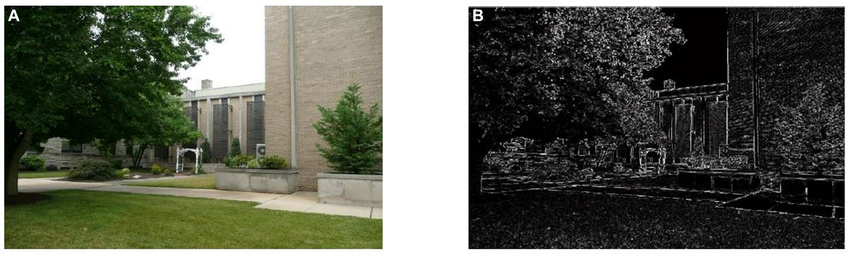
\includegraphics[width=0.8\textwidth]{image1.png}
	\caption{(A) تصویر نمونه, (B) تراکم لبه ها }
	\label{fig:results}
\end{figure}

\subsection*{\textbf{نتایج و خروجی‌ها}}
تمامی ویژگی‌های استخراج شده در فایل features.csv ذخیره شدند.
\\
- 11 ویژگی عددی برای هر تصویر
\\
- برچسب کلاس مربوطه
\\
- امکان استفاده در مراحل بعدی

\subsection*{\textbf{جمع‌بندی}}
ویژگی‌های انتخاب شده:
\\
- تفاوت بین کلاس‌های مختلف طبیعت را نشان دهند
\\
- نسبت به تغییرات جزئی در تصاویر حساس نباشند
\\
- خوب برای مراحل بعدی خوشه‌بندی 
\\
این ویژگی‌ها امکان تفکیک صحیح تصاویر طبیعی را فراهم می‌کنند.
	
\section{فاز دوم: انتخاب ویژگی‌ها}

\subsection*{\textbf{اهداف}}
هدف از فاز دوم انتخاب بهینه‌ترین ویژگی‌ها از میان 11 ویژگی استخراج شده بود. و به این منظور نیاز به ایجاد ماتریس همبستگی و تحلیل روابط بین ویژگی‌ها بود.

\subsubsection*{\textbf{محاسبه ماتریس همبستگی}}
ماتریس همبستگی به صورت دستی با استفاده از فرمول زیر محاسبه شد:
\begin{equation}
r_{xy} = \frac{\sum (x_i - \bar{x})(y_i - \bar{y})}{\sqrt{\sum (x_i - \bar{x})^2 \sum (y_i - \bar{y})^2}}
\end{equation}
برای اینکه میانگین ویژگی ها چندبار نیاز بود در ابتدا به صورت جدا حساب شد.

\subsubsection*{\textbf{معیارهای انتخاب ویژگی}}
بهترین ویژگی ها در این پروژه، ویژگی هایی هستند که کمترین همبستگی را دارند تا بتوانیم تصاویر را با معیار های متفاوت و دور از هم دسته بندی کنیم.
برای پیدا کردن بهترین ویژگی ها ابتدا داده های ماتریس را مرتب کرده و کمترین آن هارا انتخاب کردیم ولی پی بردیم که این روش خوبی نیست چون ممکن چند داده که به هم شبیه هستن انتخاب شوند. بعد جمع این مقادیر را لحاظ کردیم که باز هم روش مناسبی نبود. و در آخر از واریانس کمک گرفتیم.
\\
تابع \lr{select\_least\_k\_features} به منظور انتخاب بهینه‌ترین ویژگی‌ها برای عملیات خوشه‌بندی طراحی شده است. این تابع با ترکیب دو معیار اساسی شامل \textbf{میزان همبستگی بین ویژگی‌ها} و \textbf{میزان اطلاعات هر ویژگی}، ویژگی‌های نهایی را انتخاب می‌نماید.
\\
فرمول اصلی مورد استفاده در این تابع به صورت زیر است:

\begin{equation}
\text{امتیاز ترکیبی} = \frac{\sum|\text{همبستگی‌های ویژگی }i|}{\text{واریانس ویژگی }i}
\end{equation}
\\
این تابع در چهار گام اصلی عمل می‌کند:

\begin{enumerate}
\item محاسبه واریانس هر ویژگی به صورت جداگانه که نشان‌دهنده میزان پراکندگی و اطلاعات موجود در آن ویژگی است.

\item محاسبه مجموع قدر مطلق مقادیر همبستگی هر ویژگی با سایر ویژگی‌ها از ماتریس همبستگی که بیانگر میزان وابستگی و افزونگی آن ویژگی است.

\item محاسبه امتیاز ترکیبی برای هر ویژگی از طریق تقسیم مجموع همبستگی‌ها بر واریانس. این نسبت نشان می‌دهد که به ازای هر واحد اطلاعات، چه میزان افزونگی وجود دارد.

\item انتخاب $k$ ویژگی با کمترین امتیاز ترکیبی که بیانگر ویژگی‌های با بیشترین اطلاعات و کمترین وابستگی به سایر ویژگی‌ها است.
\end{enumerate}

\begin{figure}[h]
\centering
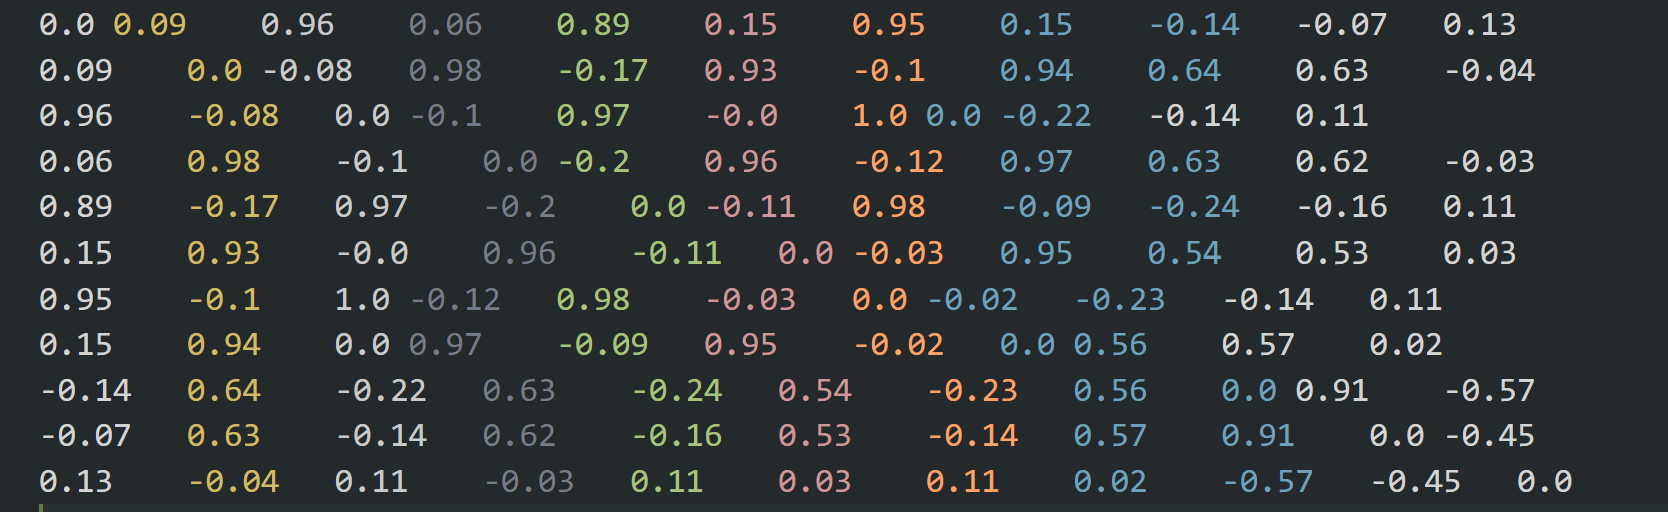
\includegraphics[width=0.8\textwidth]{correlation_matrix.png}
\caption{ماتریس همبستگی بین ویژگی‌ها}
\end{figure}


\section{فاز سوم: خوشه‌بندی}

\subsection*{\textbf{اهداف اصلی}}
\begin{itemize}
	\item پیاده‌سازی ۴ الگوریتم خوشه‌بندی مختلف
	\item تنظیم پارامترهای هر الگوریتم
	\item مقایسه عملکرد الگوریتم‌ها و انتخاب بهترین روش
	\item تحلیل ویژگی‌های متمایزکننده هر خوشه
\end{itemize}
در این فاز، پس از آماده‌سازی داده‌ها و نرمال‌سازی ویژگی‌های انتخاب شده، چهار الگوریتم خوشه‌بندی مختلف را پیاده‌سازی کردیم:

\begin{itemize}
\item \textbf{K-Means}: با تنظیم تعداد خوشه‌ها بر اساس دانش اولیه از دیتاست (۶ کلاس اصلی)
\item \textbf{Agglomerative}: با استفاده از روش پیوند کامل
\item \textbf{DBSCAN}: با پارامترهای بهینه‌شده برای شناسایی نواحی پرتراکم
\item \textbf{MeanShift}: برای شناسایی خودکار تعداد خوشه‌ها
\end{itemize}
 برای مقایسه الگوریتم ها از معیار  سیلهوئت استفاده کردیم که هرچه بیشتر باشد بهتر است.
\\
در 2 الگوریتم اخر اپسیلون و bandwidth با آزمون خطا انتخاب شد؛ اینکه بتوانند تعداد کلاستر معقولی ایجاد کنند و سیلهوئت  بالاتری ایجاد شود.
\\
DBSCAN با بالا بردن اپسیلون تعداد خوشه های معقولی ایجاد میکرد ولی شاخص کیفیت کاهش پیدا میکرد و در نهایت منفی میشد.
\\
برای meanshift با تغییر bandwidth و نزدیک 1 قرار دادن تعداد دسته های خوبی و همچنین معیار سیلهوئت  بالایی می داد اما با ادامه ی مراحل متوجه شدیم که به درستی دسته بندی نمی کند.
 \\
و براساس معیار گفته شده الگوریتم kmeans را انتخاب کردیم
\begin{figure}[h]
\centering
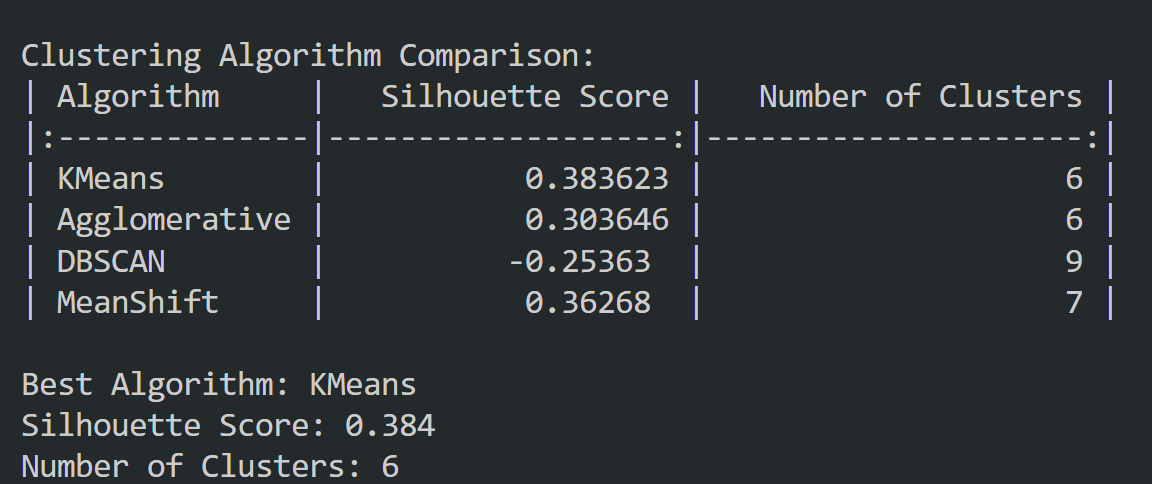
\includegraphics[width=\textwidth]{clustring_result.png}
\caption{نتایج آماری خوشه بندی}
\label{fig:clustering_results}
\end{figure}

\section{فاز چهارم: نمایش بصری نتایج الگوریتم ها}


برای مصورسازی نتایج از کتابخانه‌های زیر استفاده شده است:
\begin{itemize}
\item \textbf{Matplotlib} (نسخه 3.5.1):
\begin{itemize}
\item کتابخانه پایه برای ایجاد انواع نمودارها و ویژوال‌سازی‌ها
\item استفاده شده برای ایجاد نمودارهای پراکندگی و تنظیم جزئیات ظاهری
\end{itemize}

\item \textbf{Seaborn} (نسخه 0.11.2):
\begin{itemize}
\item کتابخانه سطح بالا مبتنی بر Matplotlib
\item استفاده شده برای ایجاد هیت‌مپ و نمودارهای پراکندگی پیشرفته
\item پالت رنگی \lr{viridis} برای نمایش بهتر خوشه‌ها
\end{itemize}
\end{itemize}


\begin{figure}[h]
\centering
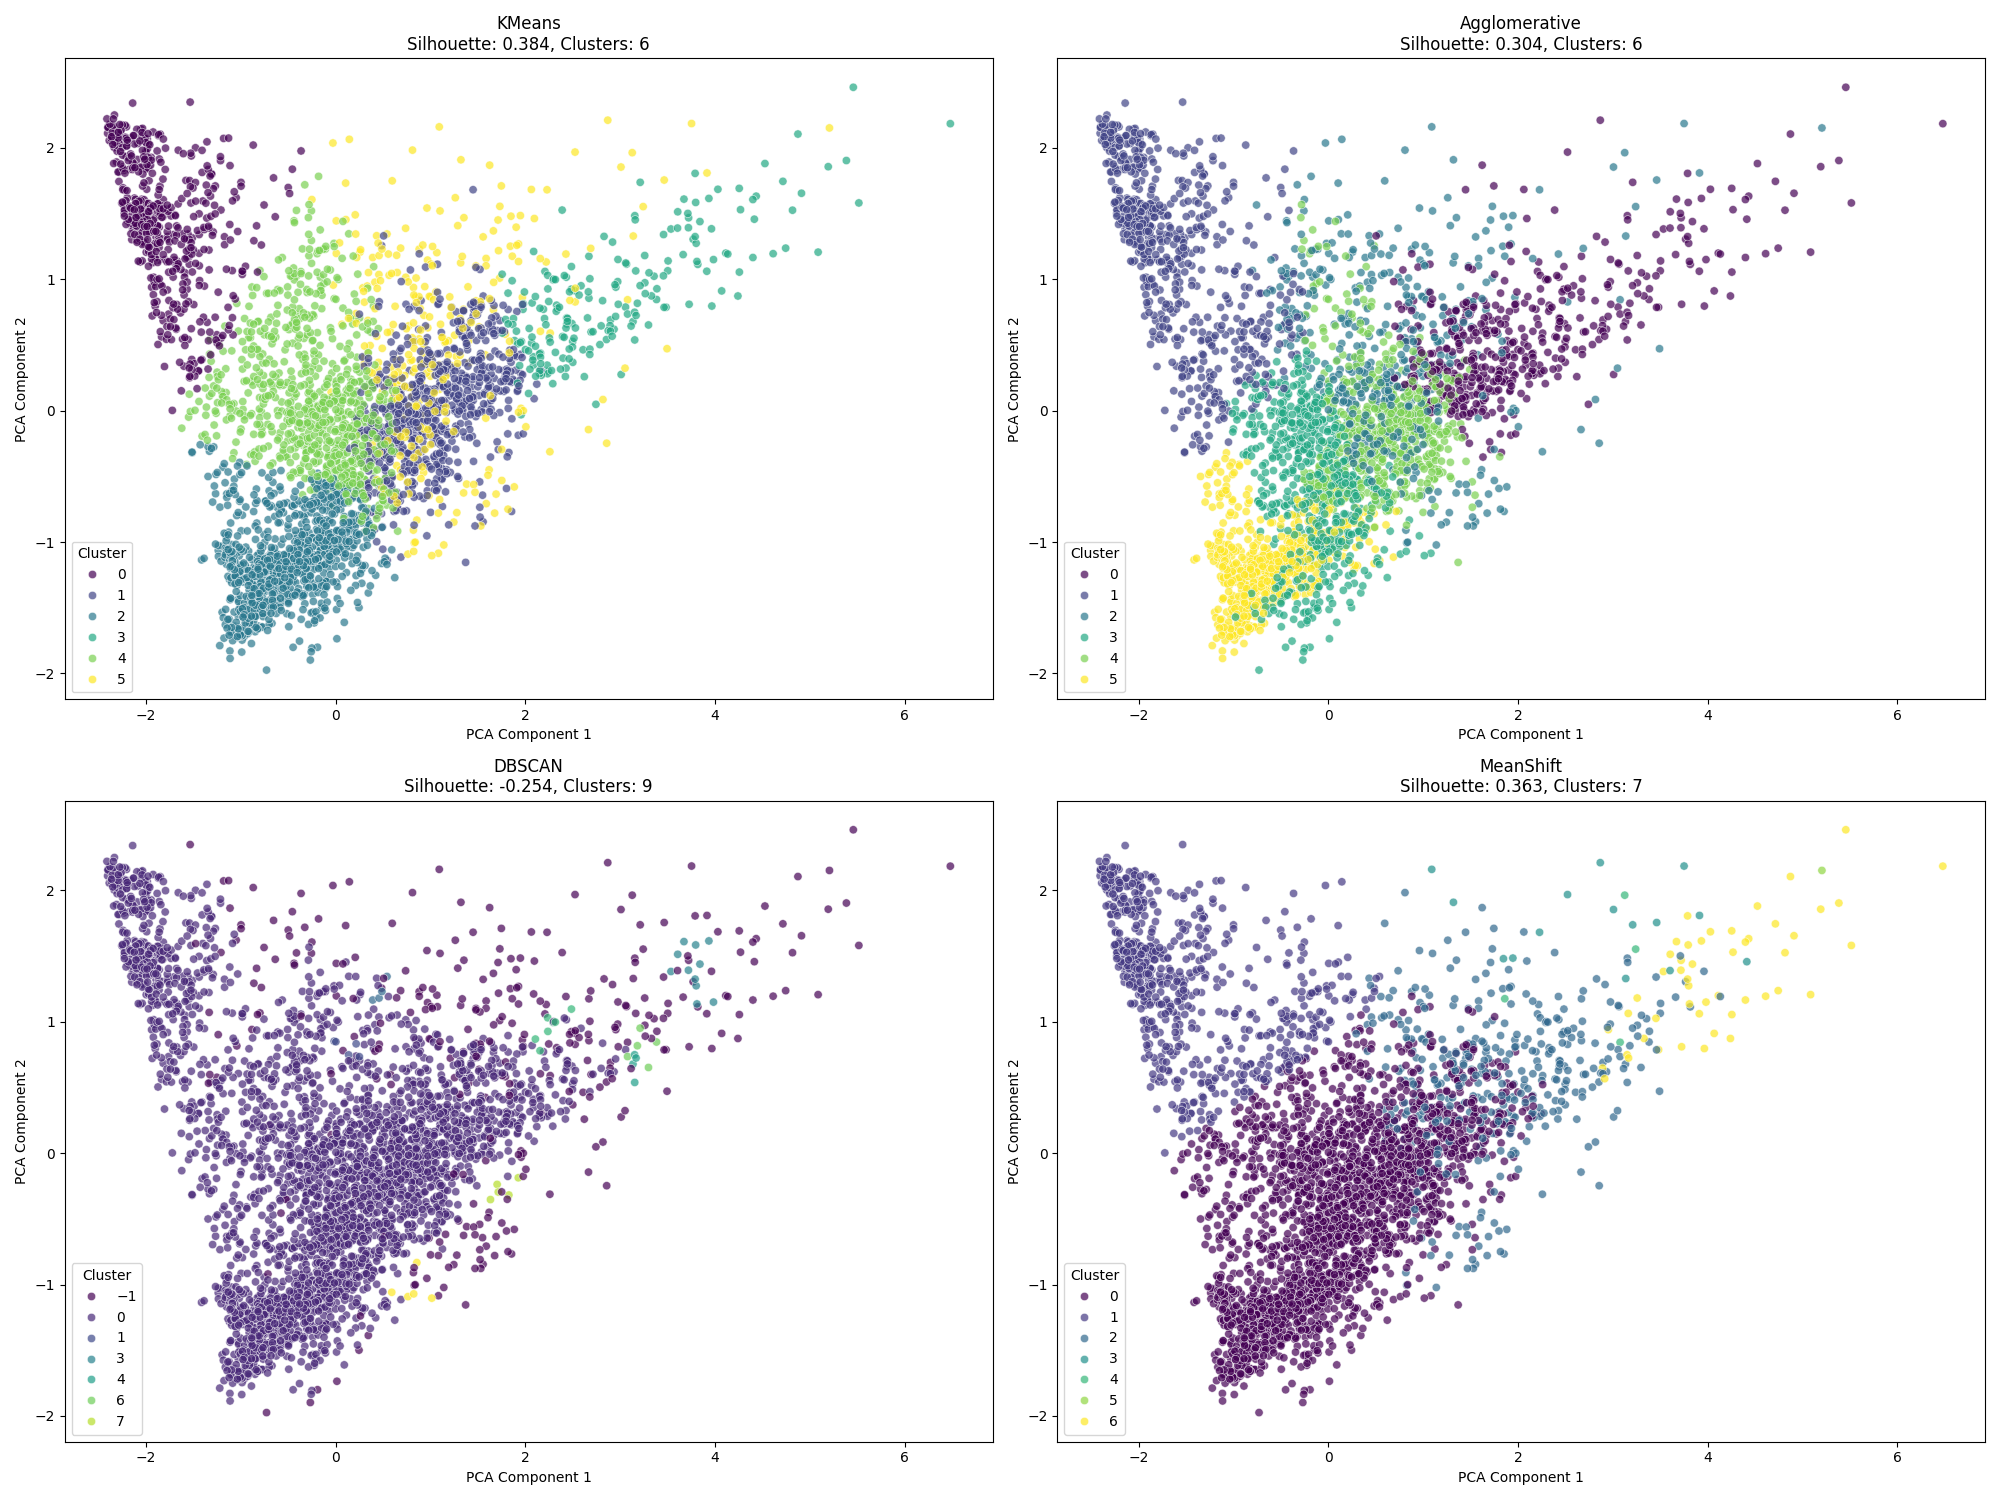
\includegraphics[width=\textwidth]{all_clustering_results.png}
\caption{نتایج خوشه‌بندی تمام الگوریتم‌ها}
\label{fig:clustering_results}
\end{figure}
	
\subsubsection*{\textbf{هیت‌مپ }}
در طراحی این هیت‌مپ، برای هر یک از خوشه‌های شناسایی‌شده، میانگین مقدار هر ویژگی محاسبه شده است. این محاسبات بر روی داده‌های استانداردشده انجام گرفته تا امکان مقایسه معنادار بین ویژگی‌های مختلف فراهم شود. مقادیر به دست آمده سپس به دامنه‌ای بین ۰ تا ۱ نرمال‌سازی شده‌اند تا تغییرات رنگ‌ها به خوبی قابل تفسیر باشند.
هیت مپ امکان شناسایی خوشه‌هایی با ویژگی‌های مشابه را فراهم کرده است و ویژگی‌های کلیدی که هر خوشه را از دیگران متمایز می‌کند، به وضوح قابل تشخیص بوده‌اند. همچنین یکنواختی یا عدم یکنواختی توزیع ویژگی‌ها در بین خوشه‌ها به راحتی قابل ارزیابی بوده است.

\clearpage
\begin{figure}[h]
\centering
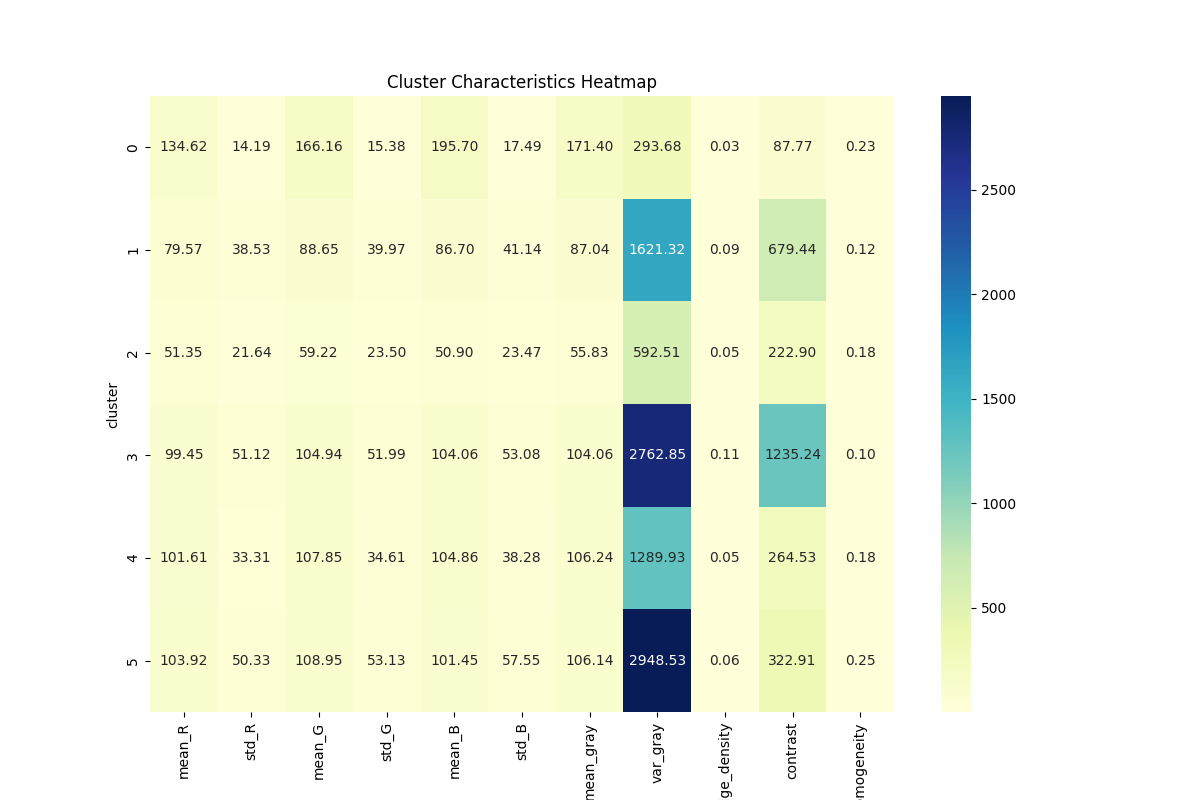
\includegraphics[width=\textwidth]{cluster_characteristics.png}
\caption{هیت مپ}
\label{fig:hitmap}
\end{figure}

	\section{فاز پنجم: ارزیابی خوشه‌بندی}
	
	\subsection*{\textbf{اهداف اصلی}}
	در این فاز، عملکرد الگوریتم‌های خوشه‌بندی با معیارهای مختلف ارزیابی شد. هدف اصلی سنجش کیفیت خوشه‌بندی انجام شده و تحلیل نتایج بود.
	\subsection*{\textbf{نتایج اجرای برنامه}}
	خروجی کنسول پس از اجرای کد:
	
	\begin{latin}
		\begin{verbatim}
			Clustering Evaluation Results:
			Average Precision: 0.5878
			Average Recall: 0.6033
			Average F1-Score: 0.5964
			Silhouette Score: 0.1472
			
			Confusion Matrix:
			Predicted 0 1 2 3 4 5
			Actual
			beach 21 18 82 0 291 188
			dense_residential 0 318 124 132 24 2
			desert 509 1 8 1 80 1
			forest 0 56 542 0 2 0
			intersection 0 283 47 67 168 35
			sea_ice 5 47 222 1 229 96
			
			Results saved to evaluation_results.csv
		\end{verbatim}
	\end{latin}
	\subsection*{\textbf{معیارهای ارزیابی}}
	
	\textbf{ Silhouette:}
	\\
	این معیار با مقدار 0.1472 نشان می‌دهد که ساختار خوشه‌بندی تا حدی مناسب است، ولی فضای بهینه‌ای بین خوشه‌ها وجود ندارد. این مقدار نشان می‌دهد که برخی نمونه‌ها نزدیک به مرز خوشه‌ها قرار گرفته‌اند.
	\\
	\textbf{ Precision:}
	\\
	با مقدار متوسط 0.5878 نشان می‌دهد که به طور متوسط حدود 58\% از نمونه‌های هر خوشه متعلق به کلاس غالب هستند. این نشان می‌دهد خوشه‌ها تا حدی خالص هستند.
	\\
	\textbf{Recall:}
	\\
	مقدار 0.6033 نشان می‌دهد که حدود 60\% از نمونه‌های هر کلاس در خوشه مربوطه قرار گرفته‌اند.
	\\
	\textbf{F1-Score:}
	\\
	با مقدار 0.5964 نشان می‌دهد که توازن نسبتاً خوبی بین دقت و فراخوانی وجود دارد.
	
	\subsection*{\textbf{تحلیل ماتریس درهم‌ریختگی}}
	- کلاس desert بهترین عملکرد را با 509 نمونه در خوشه صحیح دارد
	\\
	- کلاس beach و sea ice بیشترین اختلاط را نشان می‌دهند
	\\
	- برخی خوشه‌ها (مانند خوشه 3) نمونه‌های کمی دارند

	
	\subsection*{\textbf{تفاوت معیارها}}
	تفاوت بین مقادیر معیارها به دلایل زیر است:
	\\
	- Silhouette بر اساس فاصله‌های هندسی است
	\\
	- Precision/Recall بر اساس تطابق با برچسب‌های واقعی است
	\\
	- برخی مناطق طبیعی (مثل ساحل و یخ دریا) ویژگی‌های مشابهی دارند
	
	\subsection*{\textbf{جمع‌بندی}}
	نتایج الگوریتم خوشه‌بندی:
	\\
	- برای برخی کلاس‌ها (مانند بیابان) عملکرد خوبی دارد
	\\
	- برای کلاس‌های با ویژگی‌های مشابه نیاز به بهبود دارد
	\\
	- به طور کلی ساختار معقولی ایجاد کرده اما جای پیشرفت وجود دارد
	
	
	
	\section{فاز ششم: پیش‌بینی و تحلیل خوشه‌ها}
	
	هدف اصلی این فاز، اعمال مدل آموزش‌دیده KMeans بر روی داده‌های تست و تحلیل نتایج بود. 
ابتدا داده ها را با اسکیلر آموزش‌دیده نرمال کردیم و پیش بینی را برای 10 نمونه اجرا و در ادامه 5 نمونه ی دیگر برای هر خوشه بررسی کردیم.
\\
نتیجه خیلی دقیق نبود این به می تواند به دلیل انتخاب ویژگی ها باشد؛ چون از ویژگی های مربوط به رنگ و  کنتراست لبه ها استفاده کردیم بعضی از تصاویر به اشتباه خوشه بندی شدند.
\\
برای کلاستر 0 که مربوط به dessert هست به دلیل رنگ بسیار متفاوت و تقریبا یک دست بودن تصاویر آن، بهتر از همه خوشه بندی شده است.
\\
در کلاستر 1، تعداد عکس های مربوط به dense-residential بیشتر از بقیه است؛ اما به دلیل وجود شمایل خانه هم در dense-residential هم در intersection کمی اختلاط دارد.
\\
در کلاستر 2 که بیشتر عکس های forest است، به دلیل وجود رنگ سبز در بعضی از عکس های beach، این تصاویر هم، در این کلاستر وجود دارند. همچنین به دلیل ساختار درختان کنار هم، که شبیه به ساختار یخ ها کنار هم و همچنین ساختمان ها کنار هم ( از دور)   است بعضی از عکس های sea-ice و dense-residentail هم در این کلاستر وجود دارد.
\\
در کلاستر 3، بیشتر عکس های مربوط به intersection است ولی به دلیل گفته شده در بالا بعضی از عکس های dense-residential هم وجود دارد.
\\
کلاستر 4، مربوط به beach است؛ به دلیل وجود آب در این عکس ها و همچنین در sea-ice این دو کلاستر اختلاط دارند. به علاوه شباهت ساحل به صحرا نیز موجب وجود عکس هایی از  desert در این کلاستر شده است.
\\
کلاستر 5 هم بیشتر مربوط به sea-ice است که همانطور که گفته شد با کلاستر 4 اختلاط زیادی دارد.

\end{document}